% Created 2023-03-17 Fri 14:35
% Intended LaTeX compiler: pdflatex
\documentclass[11pt]{article}
\usepackage[utf8]{inputenc}
\usepackage[T1]{fontenc}
\usepackage{graphicx}
\usepackage{longtable}
\usepackage{wrapfig}
\usepackage{rotating}
\usepackage[normalem]{ulem}
\usepackage{amsmath}
\usepackage{amssymb}
\usepackage{capt-of}
\usepackage{hyperref}
\usepackage{minted}
\usepackage[T2A]{fontenc}
\usepackage{parskip}
\usepackage[margin=0.5in]{geometry}
\usepackage{enumerate}
\usepackage{nopageno}
\author{megabluejay}
\date{}
\title{}
\hypersetup{
 pdfauthor={megabluejay},
 pdftitle={},
 pdfkeywords={},
 pdfsubject={},
 pdfcreator={Emacs 28.2 (Org mode 9.6.1)}, 
 pdflang={English}}
\begin{document}

\begin{center}
\textbf{Лабораторная 3}

Моисеев M33001, Муров M33011
\end{center}

\begin{minted}[]{python}
import numpy as np
import matplotlib.pyplot as plt

mat = np.array([
    [1 / 3, 1 / 3, 1 / 3, 0, 0, 0, 0, 0],
    [1 / 3, 1 / 3, 1 / 3, 0, 0, 0, 0, 0],
    [0, 0, 1 / 3, 1 / 3, 0, 0, 1 / 3, 0],
    [0, 1 / 5, 0, 1 / 5, 1 / 5, 0, 1 / 5, 1 / 5],
    [0, 0, 0, 1 / 3, 1 / 3, 1 / 3, 0, 0],
    [0, 0, 0, 0, 1 / 2, 1 / 2, 0, 0],
    [0, 0, 1 / 3, 1 / 3, 0, 0, 1 / 3, 0],
    [0, 0, 0, 0, 0, 0, 1 / 2, 1 / 2],
])
\end{minted}

\begin{minted}[]{python}
eps = 1e-6
inits = [
    np.array([1, 0, 0, 0, 0, 0, 0, 0]),
    np.array([0, 1 / 2, 1 / 2, 0, 0, 0, 0, 0]),
]
results = []
for i, init in enumerate(inits):
    prev = init
    diffs = []
    while (diff := np.linalg.norm(prev - (new := prev @ mat))) >= eps:
        diffs.append(diff)
        prev = new
    results.append([round(p, 5) for p in prev])
    fig = plt.figure()
    plt.plot(diffs)
    fig.tight_layout()
    plt.savefig(f"ds{i}.png")
results
\end{minted}

\begin{center}
\begin{tabular}{rrrrrrrr}
0.04167 & 0.08333 & 0.16667 & 0.20833 & 0.125 & 0.08333 & 0.20834 & 0.08333\\[0pt]
0.04167 & 0.08333 & 0.16667 & 0.20833 & 0.125 & 0.08333 & 0.20834 & 0.08333\\[0pt]
\end{tabular}
\end{center}

\begin{figure}[htbp]
\centering
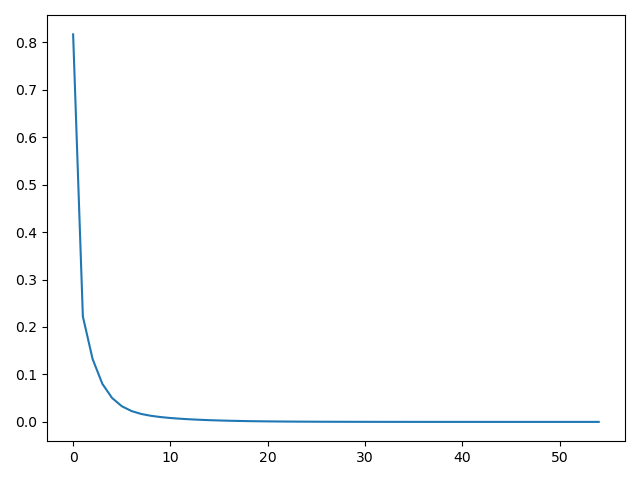
\includegraphics[width=.9\linewidth]{./ds0.png}
\caption{1 начальный вектор}
\end{figure}

\begin{figure}[htbp]
\centering
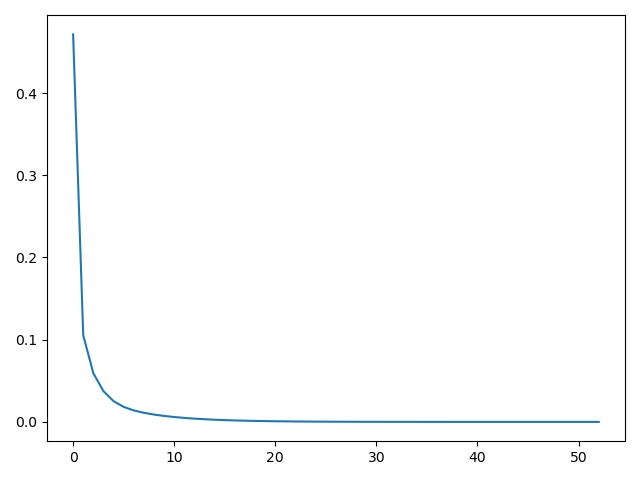
\includegraphics[width=.9\linewidth]{./ds1.png}
\caption{2 начальный вектор}
\end{figure}

\begin{minted}[]{python}
[round(p, 5) for p in np.linalg.lstsq(np.vstack([mat.T - np.eye(8), np.ones(8)]), np.ones(9))[0]]
\end{minted}

\begin{center}
\begin{tabular}{rrrrrrrr}
0.04167 & 0.08333 & 0.16667 & 0.20833 & 0.125 & 0.08333 & 0.20833 & 0.08333\\[0pt]
\end{tabular}
\end{center}
\end{document}